%% MANUSCRIPT IN THE PROGRESS IN THIS DOC: PLEASE CONTRIBUTE THERE
%%https://docs.google.com/document/d/16clK-npH8XWA7p_llKXXWScyVuvJ1bjQ9kDyP1jmniw/edit?usp=sharing

\section{Introduction}\label{sec:introduction}
In recent years, Evolutionary Algorithms (EAs) have become increasingly prominent in training agents within complex environments, particularly in areas such as video game AI \cite{lucas2006evolutionary}.
Video games serve as ideal testing grounds for EA research, as they are characterized by dynamic, non-linear challenges and uncertainties, such as unpredictable enemies \cite{togelius2007computational, togelius2009super}.
These qualities need adaptive and robust solutions, often making traditional optimization methods less effective due to high-dimensional search spaces and non-stationary conditions \cite{yannakakis2018AIgames}.
By continuously interacting with the environment, agents trained via EAs can learn to navigate and adapt to the evolving challenges posed by these complex environments.

EAs are inspired by the principles of natural selection and biological evolution, where solutions evolve over successive generations using key genetic operators such as selection, crossover (also known as recombination), and mutation \cite{eiben2015bookEA}.
These operators are essential, as they allow for the exploration and exploitation of the solution space in search of optimal solutions.
Among them, crossover and mutation are the most critical as they both contribute to genetic diversity \cite{luke1997comparison}.

Crossover, which combines genetic material from parent solutions to generate offspring, is important for exchanging successful traits between individuals in the population.
This mechanism plays a critical role in promoting the discovery of high-performing solutions by allowing favourable traits to propagate and combine in new ways.
In contrast, mutation introduces random changes to individual solutions, ensuring diversity within the generation and preventing premature convergence by exploring previously unexplored areas of the search space.
While mutation is essential for maintaining variability within the population, it typically results in incremental changes (particularly in larger populations), often refining rather than drastically improving solutions \cite{luke1997comparison}.
Given the complexity of dynamic environments, crossover plays an important role in driving the rapid improvement of solutions, creating offspring that inherit the most effective traits from different individuals, and is therefore manipulated in this study.

This study focuses on two specific crossover operators within an EA framework for training specialist agents: Blend Crossover (BLX) and Two-Point Crossover (2PX). BlLX generates offspring by producing a weighted blend of parental genes, potentially encouraging broader exploration of the solution space.
In contrast, 2PX swaps segments of genetic material between two parent solutions at two points, potentially leading to more targeted exploitation of high-performing solutions.

\subsection{Research Question and Hypotheses}
The primary objective of this study is to evaluate the effects of these two crossover operators on the performance and convergence characteristics of an EA in training a specialist agent.
Therefore two EAs are developed - EA-BLX using BLX and EA-2PX using 2PX - are developed and applied to a video game playing using a python framework called EvoMan.
This leads to the following research question:

\textit{What is the impact of BLX and 2PX on the convergence and performance of an EA in training a specialist agent in a video game playing python framework?}

\paragraph{Hypothesis 1}
EA-BLX will demonstrate a slower convergence rate than EA-2PX due to its higher exploration of the solution space.
In contrast, EA-2PX will demonstrate a faster convergence rate compared to EA-BLX due to its more exploitative nature.
\paragraph{Hypothesis 2}
Specialist agents evolved with EA-BLX will achieve higher performance compared to those evolved with EA-2PX.

\subsection{The EvoMan Framework}
The EvoMan Framework is a Python-based platform designed for evaluating evolutionary algorithms in the context of game-playing agents, specifically inspired by the boss fights from Mega Man 2 de2016electronic).
EvoMan provides an environment where specialist agents, which are optimised to face specific enemies, can be trained.
It features eight distinct enemy bosses, each with unique behaviour that present different challenges in different environments to the player agent.
Both the player and the enemies start with 100 energy points, which are reduced each time they come into contact or are hit by the weapon \cite{2016evoman}.

\section{Method}
The following section provides an overview of the crossover algorithms used and details of the experimental setup.
\subsection{Algorithm Description}
% 2 Point Crossover
\paragraph{2-Point crossover}
Two indices between 1 and $n-1$ are chosen randomly.
Both parents are split at the points specified by the indices.
The offspring is then created by glueing the split parts together, alternating between parents, which results in two children.
\begin{algorithm}
\caption{2-Point Crossover}\label{alg:2px}
\begin{algorithmic}

\Require $X^{(t)}, Y^{(t)}$
\State Choose two uniform random numbers $c_1, c_2 \in [1, n-1]$
\State $X^{(t+1)} \gets X^{(t)}[0:c_1] + Y^{(t)}[c_1:c_2] + X^{(t)}[c_2:n]$
\State $Y^{(t+1)} \gets Y^{(t)}[0:c_1] + X^{(t)}[c_1:c_2] + Y^{(t)}[c_2:n]$

\end{algorithmic}
\end{algorithm}

% Blend Crossover
\paragraph{Blend crossover}
For every pair of scalars $x_i^{(t)}, y_i^{(t)}$ from $X^{(t)}, Y^{(t)}$, respectively, a distance $d_i$ is calculated.
Using $d_i$ and the input parameter $\alpha$, an interval is constructed from which two real numbers are chosen randomly as the values for $x_i^{(t+1)}$ and $y_i^{(t+1)}$. \\
Blend crossover therefore introduces the additional hyperparameter $\alpha$ which scales the size of the interval the random values are chosen from.
\begin{algorithm}
\caption{Blend Crossover}\label{alg:blendx}
\begin{algorithmic}

\Require $X^{(t)}, Y^{(t)}$
\Ensure $\alpha \in \mathbb{R}_{\geq 0}$
\For{$i = 1, \dots, n$}
    \State $d_i \gets |x_i^{(t)} -  y_i^{(t)}|$
    \State Choose two uniform random real numbers
    \State $u_1, u_2 \in [\min(x_i^{(t)}, y_i^{(t)}) - \alpha d_i, \max(x_i^{(t)}, y_i^{(t)}) + \alpha d_i]$
    \State $x_i^{(t+1)} \gets u_1$
    \State $y_i^{(t+1)} \gets u_2$
\EndFor

\end{algorithmic}
\end{algorithm}

The two methods were chosen because they offer different advantages to the EAs.
2PX creates offspring by combining different parts of the parents.
This results in offspring that consist only of discrete genes present in their parents, which also means that they are confined to the inside of the hypercube defined by their parents.
2PX is therefore very exploitative.
BLX, on the other hand, uses the parents' genes only to define the continuous range from which the new real values are drawn.
This means that children are highly unlikely to share genes with their parents on a one-to-one basis, and also have the possibility to lie outside the parents confines.
BLX is therefore highly exploratory for a crossover operation.

\subsection{Experimental Setup}

The specific EA specifications are shown in Table 1.
The experiment consists of six training phases - three for each EA.
Both EAs are trained on the same three enemies to individually assess their performance on each one.
To optimize performance, the hyperparameters of both EAs are manually tuned throughout the experiment, using performance insights from prior runs.
They hyperparameters tuned include both standard EA parameters and those specific to each EA.
In particular, the standard deviation and mean for the Gaussian mutation, the tournament size for the tournament selection, and the $\alpha$ for BLX are adjusted.
An individual training phase consists of ten independent runs, each lasting fifty generations.
In every run one hundred initial individuals are evolved by the EA in order to maximize their fitness with respect to the chosen enemy.
Over the ten runs, the maximum fitness, average fitness and their standard deviation are recorded and the best solution is saved.
This yields two solutions for each of the three chosen enemies.

To avoid overfitting, the 'randomini' option in the EvoMan framework is set to true, which ensures that enemies start from random position.
This randomness requires the EA to account for varying enemy locations.

The EAs are trained on enemies number 2, 7 and 8.
This selection provides a diverse mix of bosses with vastly different ranges of difficulty and specialization and shows how the specialists adapt to them.

\begin{table}[tbp]
    \begin{tabu}{|l|ll|}
    \hline
    Representation            & \multicolumn{2}{l|}{Real-valued vector}                  \\ \hline
    Recombination             & \multicolumn{1}{l|}{2-PointX} & BlendX \\ \hline
    Recombination probability & \multicolumn{1}{l|}{70\%} & 70\%                         \\ \hline
    Mutation                  & \multicolumn{2}{l|}{Gaussian, $\mu$=0, $\sigma$=0.3}     \\ \hline
    Mutation probability      & \multicolumn{1}{l|}{10\%} & 5\%                          \\ \hline
    Parent selection          & \multicolumn{2}{l|}{Tournament selection, size=3}        \\ \tabucline[1.2pt]{-}
    Survival selection        & \multicolumn{2}{l|}{Replace all except best solution}    \\ \hline
    Population size           & \multicolumn{2}{l|}{100, variable}                       \\ \tabucline[1.2pt]{-}
    Number of offspring       & \multicolumn{2}{l|}{2}                                   \\ \hline
    Initialisation            & \multicolumn{2}{l|}{Random}                              \\ \hline
    Termination condition     & \multicolumn{2}{l|}{50 generations}                      \\ \hline
    \end{tabu}
    \caption{EA specification tableau.}
\end{table}

\section{Results}

\subsection{Hypothesis 1}
The results support the hypothesis that EA-BLX demonstrates a slower convergence rate compared to EA-2PX across all enemies, as it crosses the convergence threshold faster across all enemies.
The convergence threshold was defined at 85\% of the maximum fitness value, set at a fitness score of 80, where the fitness curve tends to flatten (Figure X).

For Enemy 2, EA-2PX crossed the threshold in generation 12, whereas EA-BLX crossed the threshold in generation 19.
For enemy 7, EA-2PX crossed the threshold in generation 44, whereas EA-BLX did not cross the threshold.
For Enemy 8, EA-2PX crossed the threshold twice, in generations 23 and 41, whereas EA-BLX did not cross the threshold.
Additionally, EA-BLX showed a larger standard deviation in fitness across all enemies compared to EA-2PX.

\begin{figure}[htbp]
    \centering
    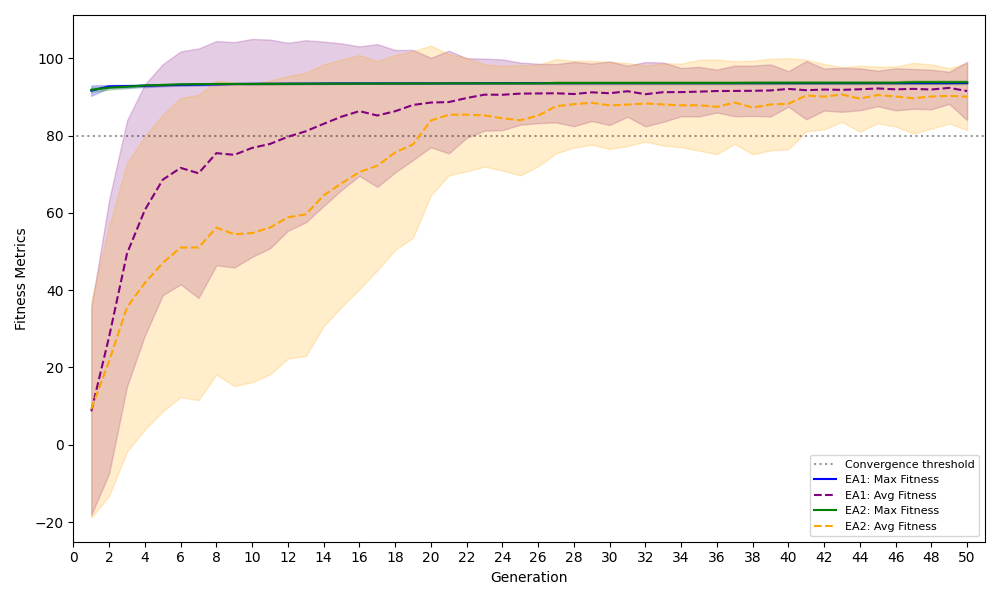
\includegraphics[width=\linewidth]{../../plots/enemy2}
    \caption{}
    \label{fig:enemy2}
\end{figure}
\begin{figure}[htbp]
    \centering
    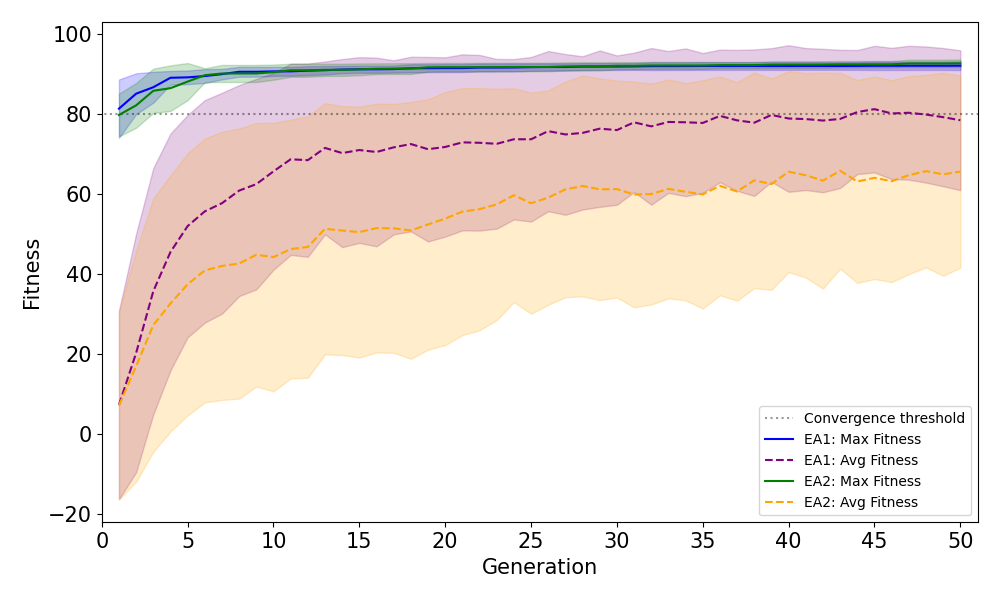
\includegraphics[width=\linewidth]{../../plots/enemy7}
    \caption{}
    \label{fig:enemy7}
\end{figure}
\begin{figure}[htbp]
    \centering
    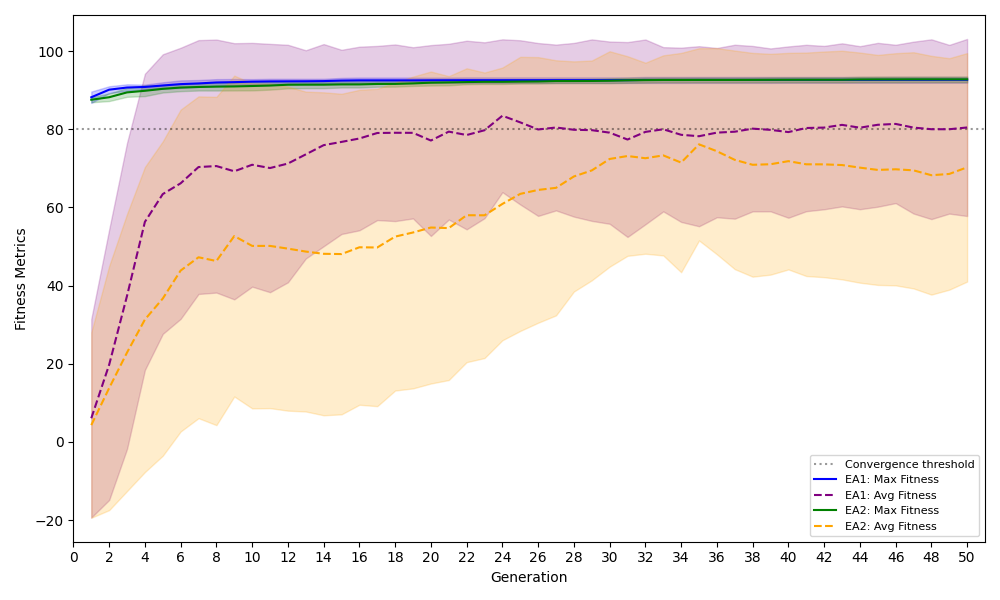
\includegraphics[width=\linewidth]{../../plots/enemy8}
    \caption{}
    \label{fig:enemy8}
\end{figure}

\subsection{Hypothesis 2}
The results partially support the hypothesis that specialist agents evolved using EA-BLX achieve higher performance compared to those evolved with EA-2PX.
Table X summarizes the maximum fitness values achieved by each EA across all three enemies.
The results indicate that for Enemy 2 and 8, EA-BLX achieved slightly higher maximum fitness values than EA1, although the differences were small - supporting the hypothesis.
In contrast, for Enemy 7, EA-2PX showed higher maximum fitness values.
Considering the SDs of the Maximum Fitness values, Enemy 7 exhibited larger SDs for both EAs.

To get more insides on the results of enemy 7, not aligning with the hypothesis, individual gains using boxplots were examined (Table X).
Given that the sample size (N = 5) limits the ability to statistically significance, the boxplot can only reveal tendencies.
The interquartile ranges (IQR) of enemy 7 reveal that 50\% of the data for both EAs fall in the same range and the means of are close to each other.
Taking the median into consideration, it can be seen that the data in EA-BLX is more evenly distributed around the median.
In contrast, EA-2PX shows a concentration of values around the median, but with two outliers that influence the IQR and the whisker.
Notably, the median for EA-2PX is higher than the median for EA-BLX, which is even negative.

\begin{table}[tbp]
    \begin{tabular}{|l|l|l|}
    \hline
    Enemy              & Crossover method & Maximum fitness \\ \hline
    \multirow{2}{*}{2} & 2-PX             & 94.14           \\ \cline{2-3}
                       & BlendX           & 94.74           \\ \hline
    \multirow{2}{*}{7} & 2-PX             & 94.64           \\ \cline{2-3}
                       & BlendX           & 94.18           \\ \hline
    \multirow{2}{*}{8} & 2-PX             & 93.71           \\ \cline{2-3}
                       & BlendX           & 93.94           \\ \hline
    \end{tabular}
\caption{Maximum achievied fitness values for each enemy and crossover method.}
\end{table}

\begin{figure}[htbp]
    \centering
    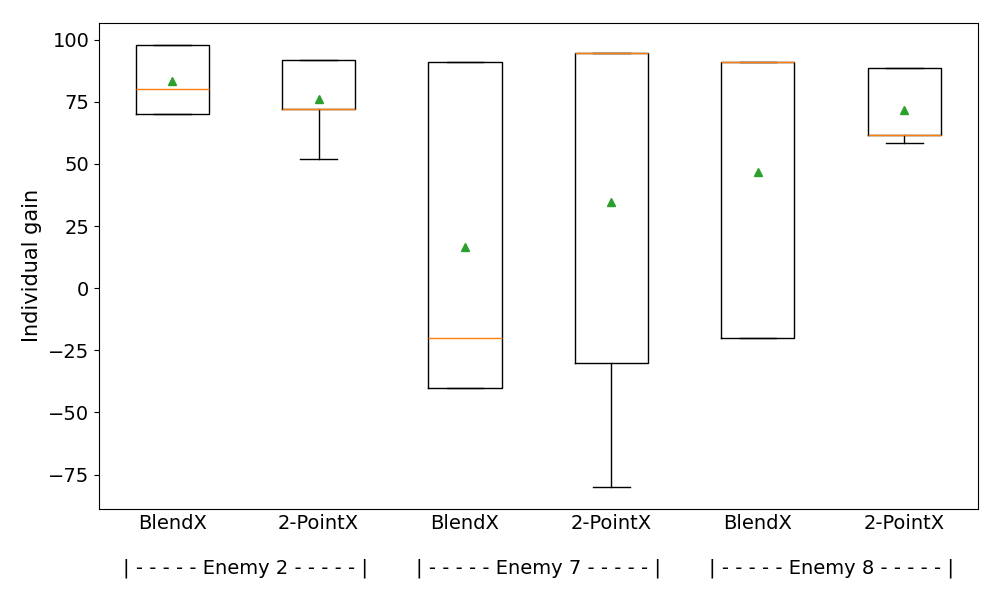
\includegraphics[width=\linewidth]{../../plots/boxplots}
    \caption{}
    \label{fig:boxplots}
\end{figure}

\section{Discussion}
The primary aim of this study was to explore the impact of BLX and 2PX on the performance and convergence characteristics of an EA when training specialist agents in a dynamic gaming environment.
The findings indicate that the 2PX operator exhibited a faster convergence rate compared to BLX.
This accelerated convergence may be attributed to the exploitative nature of 2PX, aligning with the observations of Singh and Gupta [CITE], who noted that k-point crossovers tend to capitalize on high-quality solutions.
Conversely, the BLX operator demonstrated greater variability and a slower convergence rate, which facilitated more extensive exploration and mitigated the risk of early stagnation.
This aligns with Singh and Gupta’s description of the BLX-α method as one that “creates offspring by allowing genes to vary more” [CITE], thereby preventing premature convergence and promoting higher exploration levels, as evidenced by its larger standard deviation across all enemy configurations.
In terms of specialized agent performance, the results for enemies 2 and 8 conform to the hypothesis regarding BLX's slower convergence facilitating the escape from local optima.
For enemy 7, however, a significant variability in maximum fitness outcomes is observed, which may indicate fewer local optima, thus diminishing BLX's potential advantages.
This slower convergence of BLX not only fosters greater genetic diversity but also enhances exploration, ultimately leading to improved performance.
In contrast, the rapid convergence of 2PX appears to limit genetic diversity, as it tends to exploit existing high-performing features.
To further enhance this research, future studies could benefit from programmatic optimization of hyperparameters utilizing toolboxes such as Optuna, which could refine the performance of both crossover operators.



%\section{Conclusions}

% possibly Acknowledgments or Appendices
